\documentclass[a4paper,11pt]{article}

\usepackage{amsmath}
\usepackage{fullpage}
\usepackage{bussproofs}
\usepackage{mathpartir}
\usepackage{prooftrees}
\usepackage{color}

%%% Tikz
\usetikzlibrary{calc}

\setlength{\parindent}{0pt}

\newcommand*{\equal}{=}

\newcommand*{\term}[1]{\textbf{\textit{#1}}}

\author{Sylvain Julmy}

\begin{document}

\section{Terminology}

\term{block} : a set of states, could have a \textit{representative}
states.

\term{partition} : a set of disjoint block that cover the state-space.

\section{Overview}

The bisimulation minimization algorithm has $4$ steps :
\begin{itemize}
\item Start with a sets of bad and good states.
\item Break those state into initial partition.
\item Compute the equivalence classes inside each partition.
\item Use equivalence classes as new state to check.
\end{itemize}

\begin{figure}[h]
  \centering
  \fbox{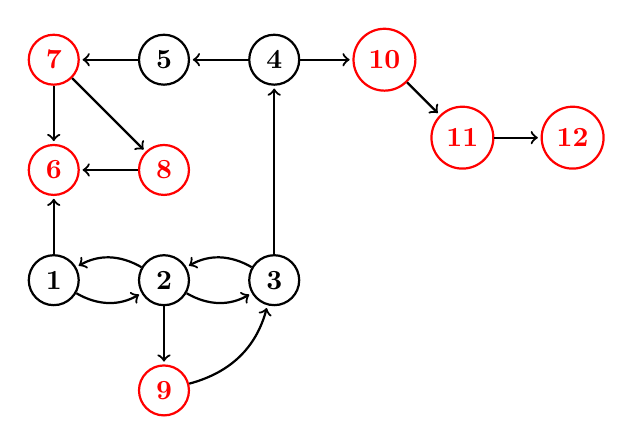
\begin{tikzpicture}[->,shorten >=1pt,auto,node distance=1.4cm,
                thick,main node/.style={circle,draw,font=\bfseries}]
	\node[main node,red] (1) {7};
	\node[main node,red] (2) [below of = 1] {6};
	\node[main node] (3) [below of = 2] {1};
	\node[main node] (4) [right of = 1] {5};
	\node[main node,red] (5) [below of = 4] {8};
	\node[main node] (6) [below of = 5] {2};
	\node[main node,red] (7) [below of = 6] {9};
	\node[main node] (8) [right of = 4] {4};
	\node[main node,red] (9) [right of = 8] {10};
	\node[main node,red] (10) [below right of = 9] {11};
	\node[main node] (11) [right of = 6] {3};
	\node[main node,red] (12) [right of = 10] {12};
	
	\path
	(1) edge node {} (2)
	(1) edge node {} (5)
	(5) edge node {} (2)
	(3) edge node {} (2)
	(6) edge [bend right] node {} (3)
	(3) edge [bend right] node {} (6)
	(6) edge node {} (7)
	(7) edge [bend right] node {} (11)
	(11) edge [bend right] node {} (6)	
	(6) edge [bend right] node {} (11)
	(11) edge node {} (8)
	(8) edge node {} (4)
	(4) edge node {} (1)
	(8) edge node {} (9)
	(9) edge node {} (10)
	(10) edge node {} (12)
;
\end{tikzpicture}}
  \caption{Initial state}
  \label{fig:bisimulation_minimization_1}
\end{figure}

\begin{figure}[h]
  \centering
  \fbox{\usetikzlibrary{calc}
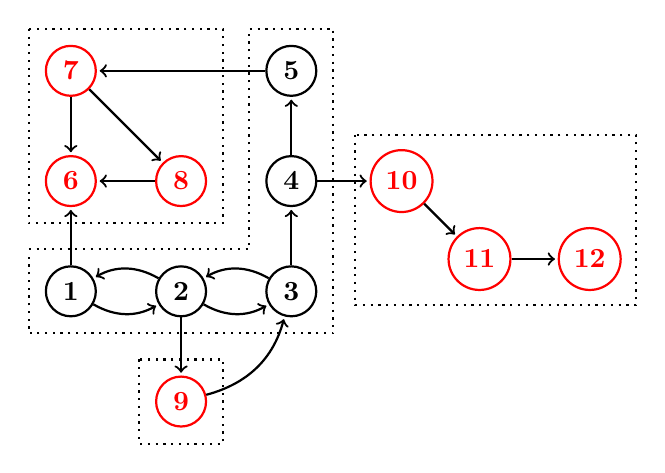
\begin{tikzpicture}[shorten >=1pt,auto,node distance=1.4cm,
                thick,main node/.style={circle,draw,font=\bfseries}]
	\node[main node,red] (1) {7};
	\node[main node,red] (2) [below of = 1] {6};
	\node[main node] (3) [below of = 2] {1};
	\node[main node,red] (5) [right of = 2] {8};
	\node[main node] (6) [below of = 5] {2};
	\node[main node,red] (7) [below of = 6] {9};
	\node[main node] (8) [right of = 5] {4};
	\node[main node] (4) [above of = 8] {5};
	\node[main node,red] (9) [right of = 8] {10};
	\node[main node,red] (10) [below right of = 9] {11};
	\node[main node] (11) [right of = 6] {3};
	\node[main node,red] (12) [right of = 10] {12};
	
	\path[->]
	(1) edge node {} (2)
	(1) edge node {} (5)
	(5) edge node {} (2)
	(3) edge node {} (2)
	(6) edge [bend right] node {} (3)
	(3) edge [bend right] node {} (6)
	(6) edge node {} (7)
	(7) edge [bend right] node {} (11)
	(11) edge [bend right] node {} (6)	
	(6) edge [bend right] node {} (11)
	(11) edge node {} (8)
	(8) edge node {} (4)
	(4) edge node {} (1)
	(8) edge node {} (9)
	(9) edge node {} (10)
	(10) edge node {} (12);
	
	\draw[black,thick,dotted] ($(1.north west)+(-0.3,0.3)$)  rectangle ($(5.south east)+(0.3,-0.3)$);
	\draw[black,thick,dotted] ($(3.north west)+(-0.3,0.3)$)  -- 
											  ($(11.north west)+(-0.3,0.3)$) --
											  ($(4.north west)+(-0.3,0.3)$) --
											  ($(4.north east)+(+0.3,0.3)$) --
											  ($(11.south east) + (0.3,-0.3)$) --
			 								  ($(3.south west)+(-0.3,-0.3)$) --
											  ($(3.north west)+(-0.3,0.3)$);
	\draw[black,thick,dotted] ($(7.north west)+(-0.3,0.3)$)  rectangle ($(7.south east)+(0.3,-0.3)$);
	\draw[black,thick,dotted] ($(9.north west)+(-0.3,0.3)$)  rectangle ($(12.south east)+(0.3,-0.3)$);

\end{tikzpicture}}
  \caption{Initial block partition}
  \label{fig:bisimulation_minimization_2}
\end{figure}

\begin{figure}[h]
  \centering
  \fbox{\usetikzlibrary{calc}
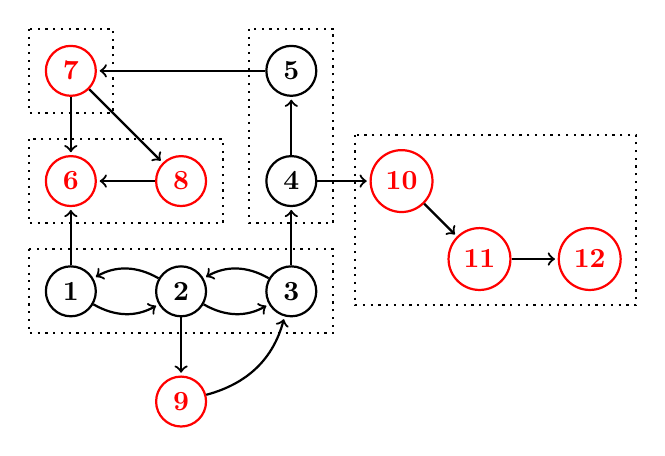
\begin{tikzpicture}[shorten >=1pt,auto,node distance=1.4cm,
                thick,main node/.style={circle,draw,font=\bfseries}]
	\node[main node,red] (1) {7};
	\node[main node,red] (2) [below of = 1] {6};
	\node[main node] (3) [below of = 2] {1};
	\node[main node,red] (5) [right of = 2] {8};
	\node[main node] (6) [below of = 5] {2};
	\node[main node,red] (7) [below of = 6] {9};
	\node[main node] (8) [right of = 5] {4};
	\node[main node] (4) [above of = 8] {5};
	\node[main node,red] (9) [right of = 8] {10};
	\node[main node,red] (10) [below right of = 9] {11};
	\node[main node] (11) [right of = 6] {3};
	\node[main node,red] (12) [right of = 10] {12};
	
	\path[->]
	(1) edge node {} (2)
	(1) edge node {} (5)
	(5) edge node {} (2)
	(3) edge node {} (2)
	(6) edge [bend right] node {} (3)
	(3) edge [bend right] node {} (6)
	(6) edge node {} (7)
	(7) edge [bend right] node {} (11)
	(11) edge [bend right] node {} (6)	
	(6) edge [bend right] node {} (11)
	(11) edge node {} (8)
	(8) edge node {} (4)
	(4) edge node {} (1)
	(8) edge node {} (9)
	(9) edge node {} (10)
	(10) edge node {} (12);

	\draw[black,thick,dotted] ($(1.north west)+(-0.3,0.3)$)  rectangle ($(1.south east)+(0.3,-0.3)$);
	\draw[black,thick,dotted] ($(2.north west)+(-0.3,0.3)$)  rectangle ($(5.south east)+(0.3,-0.3)$);
	\draw[black,thick,dotted] ($(3.north west)+(-0.3,0.3)$)  rectangle ($(11.south east)+(0.3,-0.3)$);
	\draw[black,thick,dotted] ($(4.north west)+(-0.3,0.3)$)  rectangle ($(8.south east)+(0.3,-0.3)$);
	\draw[black,thick,dotted] ($(9.north west)+(-0.3,0.3)$)  rectangle ($(12.south east)+(0.3,-0.3)$);

\end{tikzpicture}}
  \caption{Computation of equivalence classes}
  \label{fig:bisimulation_minimization_3}
\end{figure}

\begin{figure}[h]
  \centering
  \fbox{\usetikzlibrary{calc}
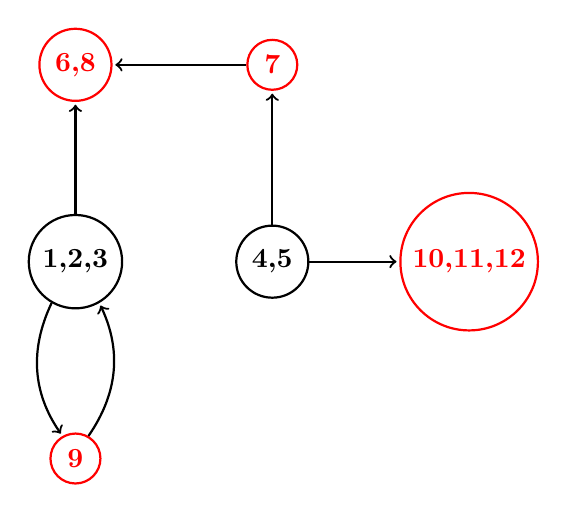
\begin{tikzpicture}[shorten >=1pt,auto,node distance=2.5cm,
                thick,main node/.style={circle,draw,font=\bfseries}]

	\node[main node,red] (1) {7};	
	\node[main node,red] (2) [left of = 1] {6,8};	
	\node[main node] (3) [below of = 2] {1,2,3};	
	\node[main node] (4) [right of = 3] {4,5};
	\node[main node,red] [below of = 3] (5) {9};
	\node[main node,red] [right of = 4] (6) {10,11,12};

	\path[->]
	(3) edge [bend right] node {} (5)
	(5) edge [bend right] node {} (3)
	(3) edge node {} (2)
	(1) edge node {} (2)
	(4) edge node {} (1)
	(4) edge node {} (6)
	;
\end{tikzpicture}}
  \caption{Final system to model-check}
  \label{fig:bisimulation_minimization_4}
\end{figure}

\section{BFH Algorithm}

Like LY, BFH selects reachable blocks to stabilize, but do not stabilize a block
the same way as LY.

\section{PT Algorithm}

\end{document}
